% Draft for IEEE PacificVis 2027 Conference Paper Track. PORT TO THE OFFICIAL IEEE VGTC TEMPLATE BEFORE SUBMISSION.
% Numbers: prototypes/paper_numbers.py (rerun after the final CDS protocol). Proofs: paper/proofs.tex (supplement).
\documentclass[10pt,twocolumn]{article}
\usepackage[margin=0.75in]{geometry}
\usepackage{amsmath,amssymb,amsthm,graphicx,booktabs,hyperref}
\newtheorem{theorem}{Theorem}\newtheorem{proposition}{Proposition}\newtheorem{corollary}{Corollary}\newtheorem{definition}{Definition}
\graphicspath{{../prototypes/output/}}
\title{How Faithful Can a Hierarchy-Constrained 1-D Layout Be?\\Certified Position--Topology Trade-offs for Merge Tree Maps and Beyond}
\author{Anonymous for review}
\date{}
\begin{document}\maketitle

\begin{abstract}
Static space--time visualizations compress each time step of a 2-D field into a 1-D column and stack columns over time. Their 1-D order is often constrained by a hierarchy: merge tree maps keep every subtree of the merge tree contiguous, and dendrogram-ordered pixel displays keep every cluster contiguous. When the hierarchy disagrees with space, every admissible layout must misplace some feature, yet existing methods measure the quality of the layout they produce rather than the error that no layout can avoid. We model such maps as hierarchy-constrained 1-D interval layouts and show that (i) the minimum achievable maximum deviation from a positional reference, $\tau^*$, has a closed form for a fixed order, decomposes into a hierarchy and a space component, and is computable at display resolution by an exact pseudo-polynomial dynamic program; (ii) for \emph{any} 1-D map and any scalar filling, breaking the contiguity of a subtree distorts merge levels by at least half the gap between the subtree's merge value and its parent's---under standard labelling conventions this distortion is the labelled interleaving distance; and (iii) together these yield a certified position--topology lower frontier. On three real datasets from two domains (two European storm winters, an Australian fire season), hierarchy-induced conflicts occur in 58--63\% of time steps under an automatic reference direction (23--77\% across fixed directions); in a geometric reader proxy, the vertical distance changes of existing merge tree maps have the opposite sign of the true approach or separation of feature pairs in 21--34\% of clear cases, and a certificate-driven relaxation lowers this to 4--15\% at a measured topological cost. The certificate also transfers to 1024-leaf dendrogram displays, where similarity hierarchies force at least 67\% of the display height of displacement.
\end{abstract}

\section{Introduction}
Static summaries show the complete evolution of spatio-temporal data in one image: Hovm\"oller diagrams in meteorology~\cite{hovmoller}, dense pixel displays and MotionRugs for movement~\cite{keim2000,motionrugs}, 1-D projections for spatio-temporal phenomena~\cite{franke2021}, and merge tree maps for time-varying scalar fields~\cite{tmtm,stmtm}. All compress space to one axis and put time on the other; readers infer spatial proximity and motion from vertical proximity.

These displays share a second property: \textbf{their 1-D order is constrained by a hierarchy}. Merge tree maps keep the leaves of every merge-tree subtree contiguous, which preserves features and the merge tree~\cite{tmtm}; clustered heatmaps~\cite{eisen1998} and hierarchical orderings of pixel displays~\cite{franke2021} keep clusters contiguous; geophylogenies align tree-constrained leaf orders with map sites~\cite{geophylo}. Hierarchy and space need not agree: two lows may merge first because they share a trough, while an unrelated third low lies geographically between them (Fig.~\ref{fig:toy}). Then every admissible layout misplaces some feature.

The visualization community has long warned that abstract views can mislead~\cite{mirages,tsne}, and projection quality is routinely measured~\cite{venna,aupetit}. ST-MTM measures distance stress and neighbourhood preservation and discusses that no 1-D order can preserve all distances~\cite{stmtm}. Such metrics describe the layout at hand. No method certifies the \emph{unavoidable} maximum deviation from a positional reference, nor states how much hierarchy information must be sacrificed to reduce it. In a geometric reader proxy on ERA5 sea-level pressure (Sec.~\ref{sec:rq2}), the vertical distance change of two lows on TMTM has the opposite sign of their true 24-h approach or separation in 33.7\% of clear cases (permutation null 39.7\%); ST-MTM, 24.9\%.

\textbf{Question.} How faithful to a positional reference can a hierarchy-constrained 1-D layout be, and can its unfaithfulness be certified, located, and controlled?

\textbf{Contributions.}
(1) A \emph{positional certificate} for hierarchy-constrained 1-D interval layouts: a closed form for fixed orders, a hierarchy/space decomposition, explanatory witness triples, and an exact pseudo-polynomial DP at display resolution (Secs.~\ref{sec:model}--\ref{sec:cert}).
(2) A \emph{filling-independent topological price} of breaking contiguity and the resulting certified \emph{position--topology lower frontier}; a threshold-and-prune relaxation whose final topological cost is measured (Sec.~\ref{sec:topo}).
(3) A \emph{cross-domain characterization} on three real and two synthetic datasets and a concrete design use on dendrogram-ordered pixel displays (Sec.~\ref{sec:eval}).

\section{Related Work}
\textbf{Static summaries.} Hovm\"oller and radius--time diagrams aggregate or slice the orthogonal dimension. Space-filling curves~\cite{franke2021,zhou2021} and pixel-oriented techniques~\cite{keim2000} linearize densely. MotionRugs~\cite{motionrugs}, stable summaries~\cite{wulms2021}, MoReVis~\cite{morevis} and GroupRugs~\cite{grouprugs} target trajectories and regions; GroupRugs keeps groups contiguous and evaluates neighbourhood-based ordering quality but gives no bound. Topological landscapes~\cite{weber2007,beketayev2012}, TMTM~\cite{tmtm} and ST-MTM~\cite{stmtm} preserve topology.
\textbf{Hierarchy-constrained orders.} Optimal leaf ordering~\cite{olo} underlies clustered heatmaps~\cite{eisen1998}; tree-constrained orders are studied for geophylogenies~\cite{geophylo}, external-order rearrangement~\cite{bulteau2022} and displacement-optimized tanglegrams~\cite{huson2026} with crossing, inversion or summed-displacement objectives.
\textbf{Faithfulness and trade-offs.} Mirages~\cite{mirages}, t-SNE misreading~\cite{tsne}, trustworthiness~\cite{venna}, distortion maps~\cite{aupetit,rauscher2026}, cartogram error trade-offs~\cite{cartograms}, data--spatial grid maps~\cite{gridmaps}, spatially ordered treemaps~\cite{wooddykes}; Meulemans argues that quality must be defined to be measured~\cite{meulemans2026}.
\textbf{1-D placement.} Without hierarchy, min--max interval separation is solvable in $O(n\log n)$~\cite{liwang}; separation-constrained QPs are used for layout~\cite{ipsep}.
\textbf{Merge tree distances.} Interleaving distances~\cite{morozov2013}, the $\ell_\infty$-cophenetic metric as labelled interleaving~\cite{munch2019}, intrinsic interleaving~\cite{gasparovic2024} and geometry-aware comparisons~\cite{yan2022}; to our knowledge they have not been used to evaluate layouts.

\section{Problem and Motivation}\label{sec:model}
\textbf{Merge tree maps.} For each time step, leaves of the merge tree (join tree for pressure minima, split tree for fire maxima) are features with extremum $R_i$, support measure $A_i$, and pairwise merge values $f(\mathrm{lca}(i,j))$. A map chooses a leaf order, an interval per leaf and an anchor (the extremum position) inside it, fills the column along leaf arcs and LCA paths~\cite{tmtm,stmtm}, and stacks columns.
\textbf{A natural remedy.} To support position tasks, anchor each feature to a reference $q_i=\varphi(R_i)$ and solve, over hierarchy-consistent orders, an LP for the smallest maximum deviation followed by a budgeted QP (reference, stress, motion residual, eccentricity). We call this the reference-anchored layout; it is part of our method.
\textbf{It is not enough.} Even the optimal anchored layout exceeds 2\% of the axis in 58\% of ERA5 frames (up to 31\%), and in the reader proxy it performs like ST-MTM (22.4\% vs 24.9\%). The obstacle is the hierarchy.

\textbf{Model.} Leaves have widths $w_i=cA_i$ ($c$ fixed over time), eccentricity radii $h_i=\rho w_i/2$, gap $g$, canvas $[a,a+L]$. A layout $(\pi,z,u)$ satisfies (H) $\pi\in\Pi(T)$, every leaf set $S_v$ contiguous; (D) $z_y-z_x\ge (w_x+w_y)/2+g$ for consecutive $x,y$; (C) $a+w_i/2\le z_i\le a+L-w_i/2$; (E) $|u_i-z_i|\le h_i$. $|\Pi(T)|=\prod_v\deg(v)!$.

\begin{figure}[t]\centering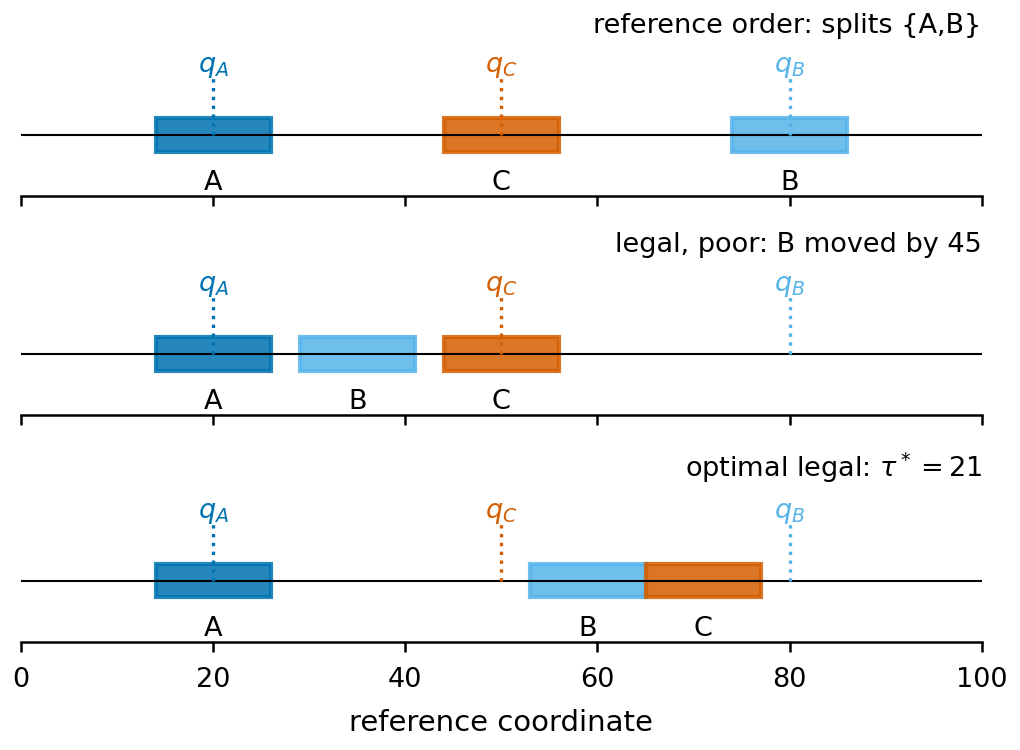
\includegraphics[width=\linewidth]{fig_toy_conflict.png}
\caption{Three-leaf conflict. Sorting by reference splits subtree $\{A,B\}$ (left); a legal but poor layout (middle); the optimal legal layout has $\tau^*=21=(q_B-q_C+w)/2$ (right).}\label{fig:toy}\end{figure}

\section{A Positional Certificate}\label{sec:cert}
\begin{definition}$\tau(\pi)=\min_{z,u}\max_i|u_i-q_i|$ s.t.\ (D)(C)(E); $\tau^*(T)=\min_{\pi\in\Pi(T)}\tau(\pi)$; $\tau_{\rm free}$ the same over all permutations; hierarchy cost $H=\tau^*-\tau_{\rm free}$.\end{definition}
\begin{proposition}[Closed form]For a fixed order with $s_k=(w_k+w_{k+1})/2+g$, $S_{ij}=\sum_{k=i}^{j-1}s_k$, $D_k=\sum_{m<k}w_m+w_k/2+(k-1)g$, $E_k=\sum_{m>k}w_m+w_k/2+(n-k)g$ and capacity $\sum w+(n-1)g\le L$: $\tau(\pi)=\max\{0,\max_{i<j}\frac{q_i-q_j+S_{ij}-h_i-h_j}{2},\max_k(a+D_k-q_k-h_k),\max_k(q_k-h_k-a-L+E_k)\}$.\end{proposition}
\begin{proposition}[Monotonicity, witness]Flattening nodes never increases $\tau^*$; flattening all gives $\tau_{\rm free}$, so $H\ge0$. If $i,j\in S_v$, $k\notin S_v$, $q_i<q_k<q_j$, then $\tau^*\ge\frac12\min(q_k-q_i,q_j-q_k)$.\end{proposition}
\begin{theorem}[Exact DP]At pixel resolution with integer widths $W_i$ and gap $G$, let $E_S(x)$ be the earliest next start after placing subtree $S$ with all starts $\ge x$. Then $E_{\rm leaf}(x)=\max(x,lo_i)+W_i+G$ (or $\infty$), $E_S=\min(E_B\circ E_A,E_A\circ E_B)$ for binary nodes (subset DP for $m$-ary), and $\tau$ is feasible iff $E_{\rm root}(0)<\infty$. Bisection gives $\tau^*$ to tolerance in $O(nN\log)$ for binary trees (pseudo-polynomial in $N$; $O(2^m mN)$ per $m$-ary node).\end{theorem}
\begin{proposition}[Certified lower bound]Rounding widths and gap down while keeping the slacks gives $\tau^*_{\rm cont}\ge\tau^*_{\rm disc,relax}-\delta/2$; with integer widths, $0\le\tau^*_{\rm disc}-\tau^*_{\rm cont}\le\delta/2$.\end{proposition}
Numerically, the closed form matches LP to $2\cdot10^{-14}$; the DP matches brute force on 300 random hierarchies within 0.495\,px; 4096 leaves take 4\,s. The scalable part is the certificate; selecting a layout inside the budget still enumerates candidate orders.

\section{The Price of Topology}\label{sec:topo}
For any function $g$ on the line with anchors $a_i$, let $m_g(i,j)=\max_{[a_i,a_j]}g$ (join tree) and $d_{\rm top}=\max_{i\ne j}|m_g(i,j)-f(\mathrm{lca}_T(i,j))|$. With bijective leaf labels, equal leaf heights and no additional extrema, $d_{\rm top}$ is the labelled interleaving distance~\cite{munch2019}.
\begin{theorem}[Topological price of non-contiguity]If the leaf set of a non-root node $v$ is not contiguous in a 1-D map, then for any filling $d_{\rm top}\ge\gamma_v/2$, $\gamma_v=f(p(v))-f(v)$; the factor $1/2$ is tight in general.\end{theorem}
\begin{proof}[Sketch]Take $i,j\in S_v$ and $k\notin S_v$ between them: $m_g(i,k)\le m_g(i,j)$, while $m_T(i,j)\le f(v)$ and $m_T(i,k)\ge f(p(v))$; summing the three differences gives $\gamma_v\le2d_{\rm top}$.\end{proof}
\begin{corollary}[Lower frontier]With $\Phi_T(\delta)=\tau^*(T$ with all nodes of $\gamma_v\le2\delta$ flattened$)$, every layout and filling satisfies $\max_i|u_i-q_i|\ge\Phi_T(d_{\rm top})$. The bound is necessary, not generally attainable.\end{corollary}
\textbf{Relaxation.} In frames with $H>\theta$ we flatten all nodes with $\gamma_v\le\kappa$ and prune flattenings (strongest first) whose removal does not raise $\tau^*$; this handles plateaus where only a set of flattenings helps. $\kappa$ selects nodes; the final $d_{\rm top}$ is measured. With LCA filling, $d_{\rm top}/\max\gamma$ has median 1.0--1.23 and maximum 2.94; we claim no approximation guarantee.
\textbf{Defaults.} Reference = principal direction of tracked extremum motion; width scale maps the domain area to half the axis; $g=L/240$, $\Delta=L/120$, $\rho=.5$; single legibility constant $\theta=2\%$ of the axis.

\section{Evaluation}\label{sec:eval}
\textbf{Data.} ERA5 MSLP Europe 1999-11-17..2000-01-14 (118 frames, 12\,h) and 2013-12..2014-01 (124 frames), following the protocol of the reference-anchored layout (equal-area projection, 250\,km smoothing, $49\times49$); Australian fire radiative power (10\,km, Nov--Dec 2019, 2-day sums, 30 frames, $\log(1+{\rm FRP})$, smallest smoothing giving $\le12$ maxima); Ring~\cite{tmtm,franke2021}; a replica of ST-MTM's three-Gaussian scene. Baselines: TMTM, ST-MTM (adapted defaults outside Ring), fixed-$x$ anchoring; ours with topology kept (A) and relaxed (R).

\textbf{RQ1: prevalence.} $H>\theta$ in 58\% / 60\% / 63\% of frames (ERA5 / ERA5-2014 / fire) under the automatic direction and 23--77\% across eight fixed directions; max $H$ 31\% / 38\% / 20\% of the axis; space cost $<5\%$ (Fig.~\ref{fig:overview}).

\begin{figure*}[t]\centering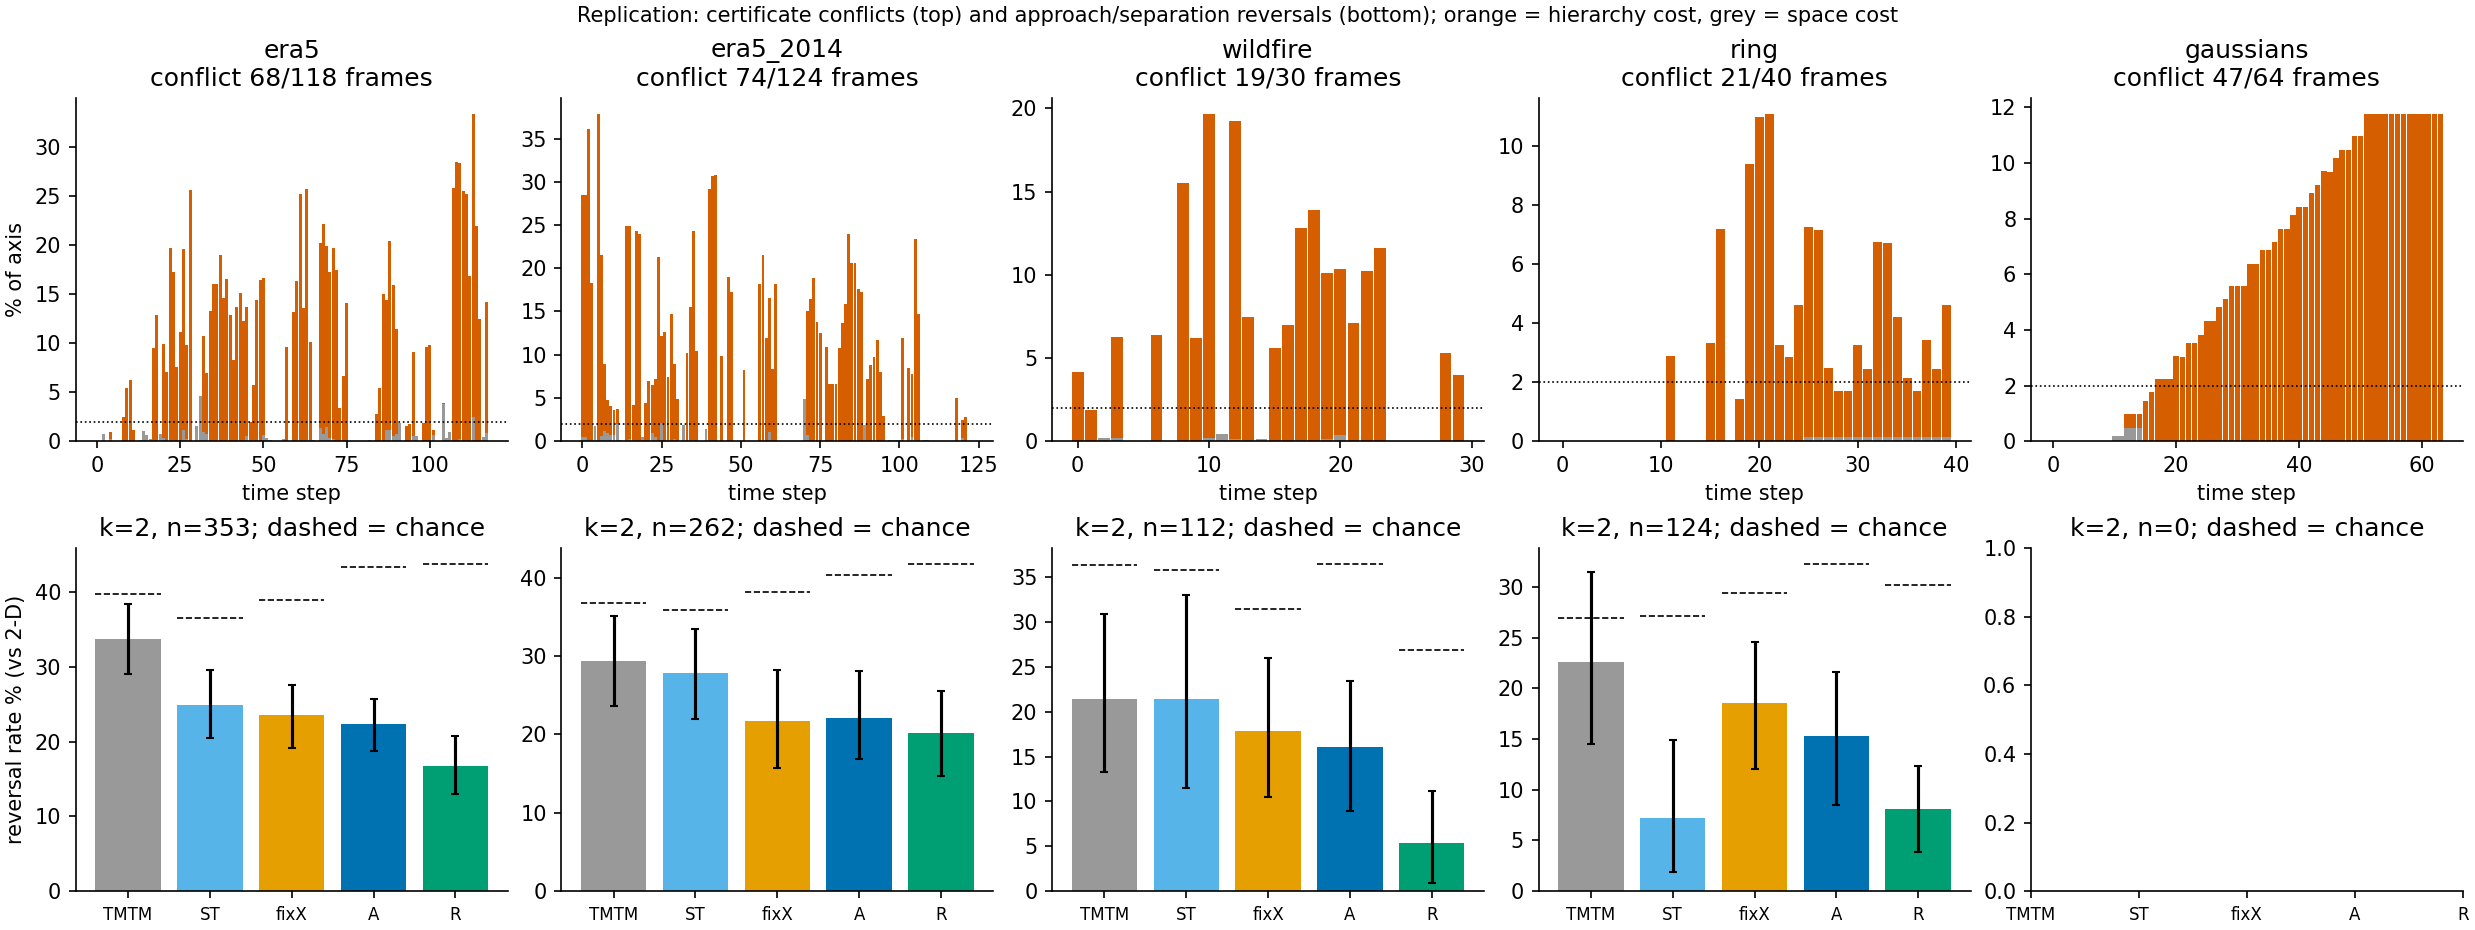
\includegraphics[width=\textwidth]{replicate_overview.png}
\caption{Top: per-frame space cost (grey) and hierarchy cost (orange). Bottom: sign-disagreement rates of the geometric reader proxy (95\% CI); dashed: permutation null.}\label{fig:overview}\end{figure*}

\textbf{RQ2: geometric reader proxy.}\label{sec:rq2} A pair's map distance change beyond 2\% of the occupied anchor range is read as approach/separation; truth is the 2-D extremum distance change beyond 2\% of the diagonal. Table~\ref{tab:proxy} reports reversals (clear opposite) and misses; differences use a paired 8-frame block bootstrap. R reverses significantly less than ST-MTM on all three real datasets (differences $-11.9$, $-13.0$, $-17.9$ points, CIs excluding 0) but misses more on fire ($+15.2$ points). Ring shows no significant difference. The ranking holds for reader thresholds of 1/2/5\%. This is a geometric diagnostic, not a human study.

\begin{table}[t]\centering\small
\begin{tabular}{lrcccc}\toprule
data & $n$ & TMTM & ST-MTM & A & R\\\midrule
ERA5 & 353 & 33.7 & 24.9 / 27.2 & 22.4 / 9.3 & \textbf{13.0} / 7.1\\
ERA5-14 & 262 & 29.4 & 27.9 / 26.7 & 22.1 / 17.2 & \textbf{14.9} / 17.9\\
Fire & 112 & 21.4 & 21.4 / 14.3 & 16.1 / 16.1 & \textbf{3.6} / 29.5\\
Ring & 124 & 22.6 & \textbf{7.3} / 27.4 & 24.2 / 7.3 & 10.5 / 2.4\\\bottomrule
\end{tabular}
\caption{Reversal / miss rates (\%), 24-h (fire: 4-day) windows.}\label{tab:proxy}\end{table}

\textbf{RQ3: cost and frontier.} Fig.~\ref{fig:frontier}: no achieved point lies below the certified frontier; Theorem~2 holds in all 924 frames with broken contiguity and the corollary in every frame. At $\kappa=2\%$ of the value range the mean reference error drops 11--13\% on pressure (2.5--2.7\,hPa) but 45\% on fire; at $\kappa=20\%$, 59--74\% on pressure at 28--33\,hPa. The cost of fidelity depends on the merge structure.

\begin{figure*}[t]\centering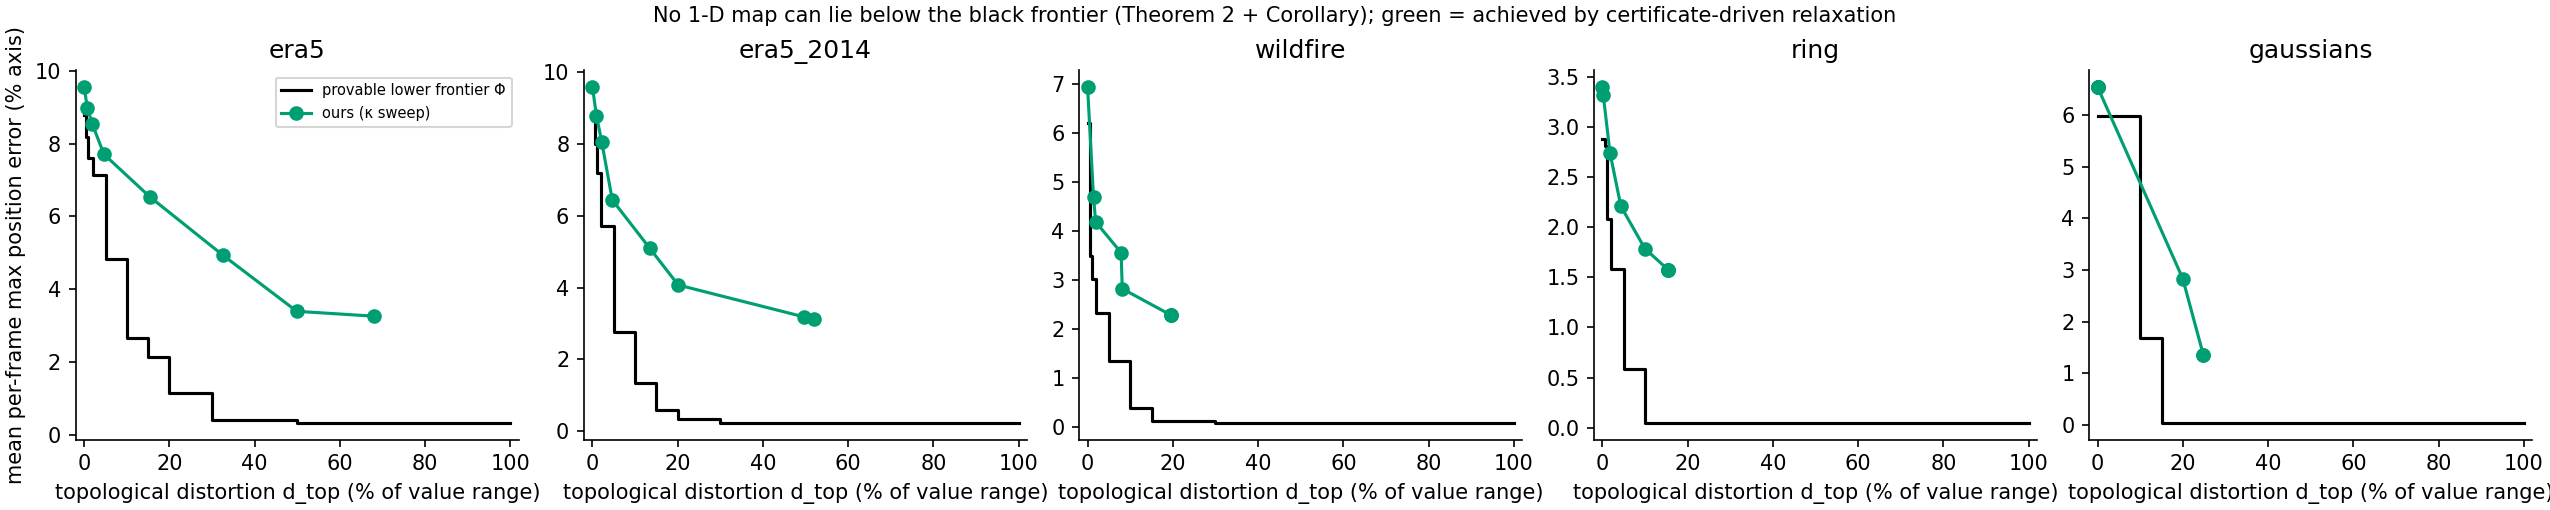
\includegraphics[width=\textwidth]{frontier.png}
\caption{Certified position--topology lower frontier (black) and achieved layouts (green points).}\label{fig:frontier}\end{figure*}

\textbf{RQ4: dendrogram displays.} For 1024 fire cells ordered by an OLO dendrogram of their FRP time series, cells sit up to 88\% of the display height from their geographic position (median 14\%); the certificate proves that no dendrogram-consistent order goes below 67\% (Fig.~\ref{fig:dendro}), so the reading ``row position $\approx$ geography'' is untenable; a spatial Ward dendrogram costs only 1.4\% (hierarchy cost).

\begin{figure*}[t]\centering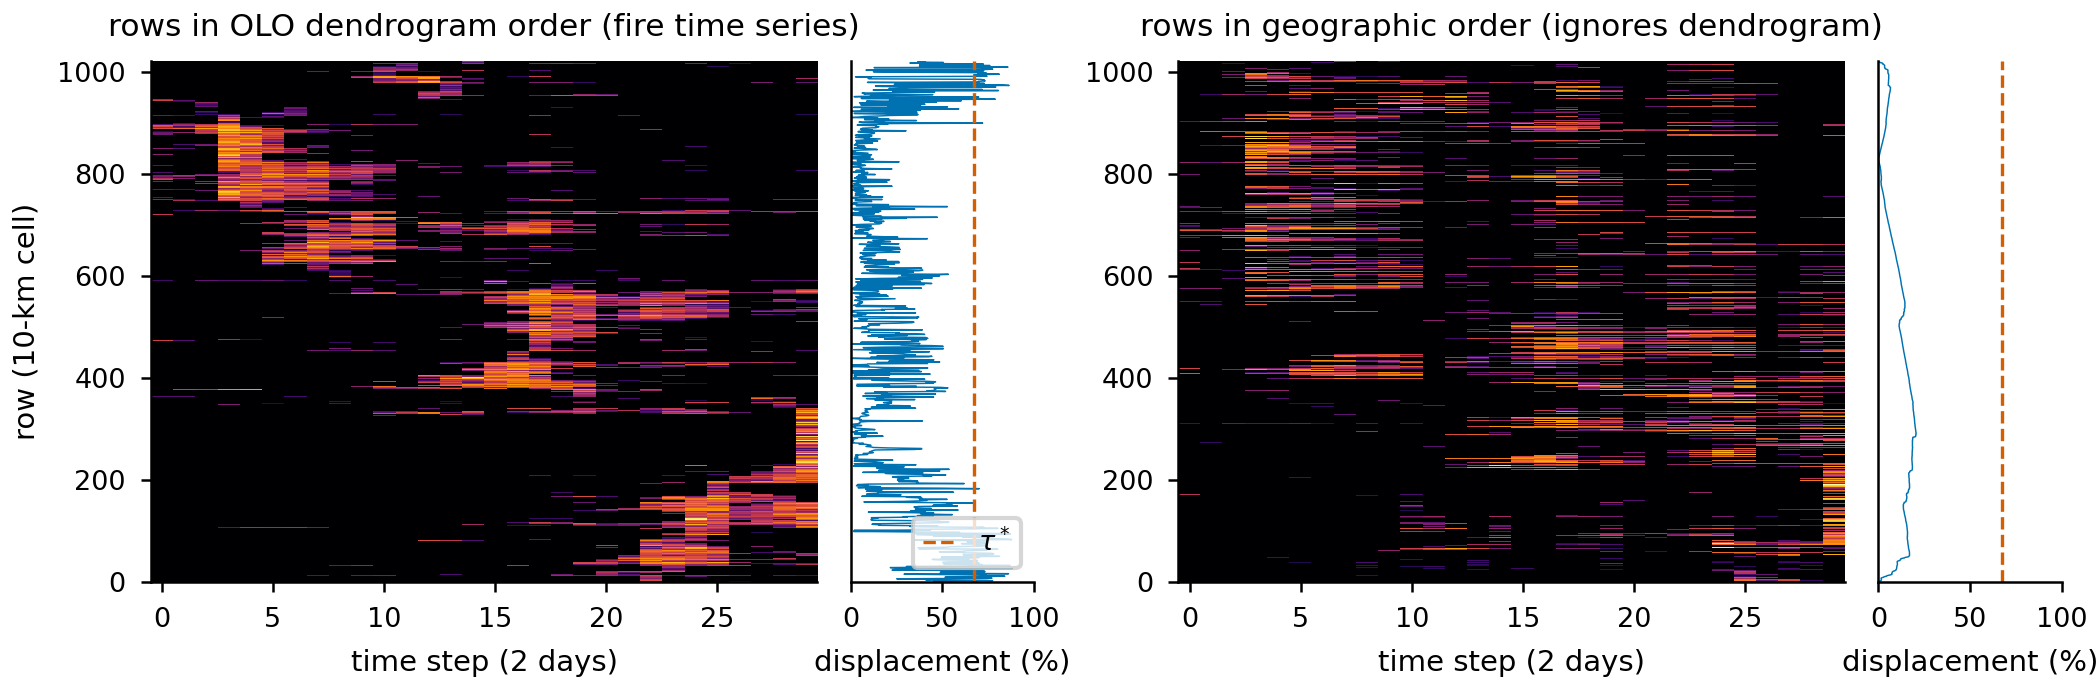
\includegraphics[width=\textwidth]{dendrogram_demo.png}
\caption{Dendrogram-ordered pixel display of 1024 fire cells: OLO order (left) vs.\ geographic order (right), with per-row displacement and the certificate $\tau^*$.}\label{fig:dendro}\end{figure*}

\section{Discussion and Limitations}
Default to preserving the hierarchy and disclose the certified deviation; relax explicitly when position matters and show the cost; report achieved error relative to the certificate when proposing layouts. Limitations: the reader proxy is geometric; baselines are evaluated in our interval model (native width models pending); relaxation has no approximation guarantee; the DP is pseudo-polynomial and exponential in node degree, and layout selection still enumerates; ERA5 from the ARCO mirror (to be rerun on CDS); one reference direction cannot encode orthogonal motion. Negative results: automatic radial centres follow tracking artefacts; a stability-priority policy did not generalize; per-feature disclosure ticks were illegible on ERA5.

\section{Conclusion}
We certified how far hierarchy-constrained 1-D layouts must deviate from a positional reference, proved a filling-independent topological price for breaking contiguity, and derived a certified position--topology frontier. Across two domains, hierarchy conflicts are common and their resolution cost depends on the merge structure.

\begin{thebibliography}{99}\small
% TODO: /aris:citation-audit before submission
\bibitem{tmtm} W.~K\"opp, T.~Weinkauf. Temporal merge tree maps. IEEE TVCG 29(1), 2023.
\bibitem{stmtm} Spatiotemporal merge tree maps. Preprint, SSRN 6604235, 2026.
\bibitem{franke2021} M.~Franke et al. Visual analysis of spatio-temporal phenomena with 1D projections. CGF 40(3), 2021.
\bibitem{zhou2021} L.~Zhou, C.~R.~Johnson, D.~Weiskopf. Data-driven space-filling curves. IEEE TVCG 27(2), 2021.
\bibitem{hovmoller} E.~Hovm\"oller. The trough-and-ridge diagram. Tellus 1(2), 1949.
\bibitem{keim2000} D.~A.~Keim. Designing pixel-oriented visualization techniques. IEEE TVCG 6(1), 2000.
\bibitem{motionrugs} J.~Buchm\"uller et al. MotionRugs. IEEE TVCG, 2019.
\bibitem{wulms2021} J.~Wulms et al. Stable visual summaries for trajectory collections. PacificVis, 2021.
\bibitem{morevis} G.~Valdrighi et al. MoReVis. IEEE TVCG 30(4), 2024.
\bibitem{grouprugs} M.~C.~A.~Stolk, J.~J.~H.~M.~Wulms, K.~A.~B.~Verbeek. GroupRugs. PacificVis, 2025.
\bibitem{weber2007} G.~H.~Weber, P.-T.~Bremer, V.~Pascucci. Topological landscapes. IEEE TVCG 13(6), 2007.
\bibitem{beketayev2012} K.~Beketayev et al. Geometry-preserving topological landscapes. WASA, 2012.
\bibitem{olo} Z.~Bar-Joseph, D.~K.~Gifford, T.~S.~Jaakkola. Fast optimal leaf ordering. Bioinformatics 17, 2001.
\bibitem{eisen1998} M.~B.~Eisen et al. Cluster analysis and display of genome-wide expression patterns. PNAS 95(25), 1998.
\bibitem{geophylo} J.~Klawitter et al. Visualizing geophylogenies. GIScience 2023 / JGAA 2025.
\bibitem{bulteau2022} L.~Bulteau, P.~Gambette, O.~Seminck. Reordering a tree according to an order on its leaves. CPM, 2022.
\bibitem{huson2026} D.~H.~Huson. Displacement-optimized tanglegrams. MBE 43(3), 2026.
\bibitem{mirages} A.~McNutt, G.~Kindlmann, M.~Correll. Surfacing visualization mirages. CHI, 2020.
\bibitem{tsne} M.~Wattenberg, F.~Vi\'egas, I.~Johnson. How to use t-SNE effectively. Distill, 2016.
\bibitem{venna} J.~Venna, S.~Kaski. Neighborhood preservation in nonlinear projection methods. ICANN, 2001.
\bibitem{aupetit} M.~Aupetit. Visualizing distortions and recovering topology in continuous projection techniques. Neurocomputing 70, 2007.
\bibitem{rauscher2026} J.~Rauscher et al. Visual boosting techniques for spatiotemporal dense pixel visualizations. EuroVA, 2026.
\bibitem{cartograms} S.~Nusrat, S.~Kobourov. The state of the art in cartograms. CGF 35(3), 2016.
\bibitem{gridmaps} N.~van Beusekom et al. Data-spatial layouts for grid maps. GIScience, 2023.
\bibitem{wooddykes} J.~Wood, J.~Dykes. Spatially ordered treemaps. IEEE TVCG 14(6), 2008.
\bibitem{meulemans2026} W.~Meulemans. An algorithmic perspective on information visualization. arXiv:2607.29360, 2026.
\bibitem{liwang} S.~Li, H.~Wang. Separating overlapped intervals on a line. JoCG 10(1), 2019.
\bibitem{ipsep} T.~Dwyer, Y.~Koren, K.~Marriott. IPSep-CoLa. IEEE TVCG 12(5), 2006.
\bibitem{morozov2013} D.~Morozov, K.~Beketayev, G.~H.~Weber. Interleaving distance between merge trees. TopoInVis, 2013.
\bibitem{munch2019} E.~Munch, A.~Stefanou. The $\ell_\infty$-cophenetic metric for phylogenetic trees as an interleaving distance. 2019.
\bibitem{gasparovic2024} E.~Gasparovic et al. Intrinsic interleaving distance for merge trees. La Matematica, 2024.
\bibitem{yan2022} L.~Yan et al. Geometry-aware merge tree comparisons for time-varying data with interleaving distances. IEEE TVCG, 2022.
\end{thebibliography}
\end{document}
